% Options for packages loaded elsewhere
\PassOptionsToPackage{unicode}{hyperref}
\PassOptionsToPackage{hyphens}{url}
%
\documentclass[
  8pt,
  ignorenonframetext,
]{beamer}
\usepackage{pgfpages}
\setbeamertemplate{caption}[numbered]
\setbeamertemplate{caption label separator}{: }
\setbeamercolor{caption name}{fg=normal text.fg}
\beamertemplatenavigationsymbolsempty
% Prevent slide breaks in the middle of a paragraph
\widowpenalties 1 10000
\raggedbottom
\setbeamertemplate{part page}{
  \centering
  \begin{beamercolorbox}[sep=16pt,center]{part title}
    \usebeamerfont{part title}\insertpart\par
  \end{beamercolorbox}
}
\setbeamertemplate{section page}{
  \centering
  \begin{beamercolorbox}[sep=12pt,center]{part title}
    \usebeamerfont{section title}\insertsection\par
  \end{beamercolorbox}
}
\setbeamertemplate{subsection page}{
  \centering
  \begin{beamercolorbox}[sep=8pt,center]{part title}
    \usebeamerfont{subsection title}\insertsubsection\par
  \end{beamercolorbox}
}
\AtBeginPart{
  \frame{\partpage}
}
\AtBeginSection{
  \ifbibliography
  \else
    \frame{\sectionpage}
  \fi
}
\AtBeginSubsection{
  \frame{\subsectionpage}
}
\usepackage{amsmath,amssymb}
\usepackage{lmodern}
\usepackage{iftex}
\ifPDFTeX
  \usepackage[T1]{fontenc}
  \usepackage[utf8]{inputenc}
  \usepackage{textcomp} % provide euro and other symbols
\else % if luatex or xetex
  \usepackage{unicode-math}
  \defaultfontfeatures{Scale=MatchLowercase}
  \defaultfontfeatures[\rmfamily]{Ligatures=TeX,Scale=1}
\fi
% Use upquote if available, for straight quotes in verbatim environments
\IfFileExists{upquote.sty}{\usepackage{upquote}}{}
\IfFileExists{microtype.sty}{% use microtype if available
  \usepackage[]{microtype}
  \UseMicrotypeSet[protrusion]{basicmath} % disable protrusion for tt fonts
}{}
\makeatletter
\@ifundefined{KOMAClassName}{% if non-KOMA class
  \IfFileExists{parskip.sty}{%
    \usepackage{parskip}
  }{% else
    \setlength{\parindent}{0pt}
    \setlength{\parskip}{6pt plus 2pt minus 1pt}}
}{% if KOMA class
  \KOMAoptions{parskip=half}}
\makeatother
\usepackage{xcolor}
\newif\ifbibliography
\setlength{\emergencystretch}{3em} % prevent overfull lines
\providecommand{\tightlist}{%
  \setlength{\itemsep}{0pt}\setlength{\parskip}{0pt}}
\setcounter{secnumdepth}{-\maxdimen} % remove section numbering
% type setting
% ------------------------------------------------------------------------------
\usepackage[german]{babel}     

% fonts
% ------------------------------------------------------------------------------
\usefonttheme{professionalfonts}

% slide title and horizontal line
% ------------------------------------------------------------------------------
\setbeamertemplate{frametitle}{%
    \vskip-30pt \color{black}\large%
    \begin{minipage}[b][23pt]{120mm}%
    \flushleft\insertframetitle%
    \end{minipage}%
}

\setbeamertemplate{headline}										
{
\vskip10pt\hfill\hspace{3.5mm} 										 
\vskip15pt\color{black}\rule{\textwidth}{0.4pt} 					 
}

% slide number
% ---------------------------------------------------------------
\setbeamertemplate{navigation symbols}{}
\setbeamertemplate{footline}
{
\vskip5pt
\vskip2pt
\makebox[123mm]{\hspace{7.5mm}
\hfill Wahrscheinlichkeitstheorie und Frequentistische Inferenz $\vert$ 
\copyright $ $ 2023 Dirk Ostwald CC BY-SA 4.0 $\vert$ 
Folie \insertframenumber}
\vskip4pt
}

% block color scheme
% ------------------------------------------------------------------------------
% colors
\definecolor{white}{RGB}{255,255,255}
\definecolor{grey}{RGB}{235,235,235}
\definecolor{lightgrey}{RGB}{245,245,245}
\definecolor{LightBlue}{RGB}{220,220,255}
\definecolor{darkblue}{RGB}{51, 51, 153}

% definitions and theorems
\setbeamercolor{block title}{fg = black, bg = grey}
\setbeamercolor{block body}{fg = black, bg = lightgrey}

% general line spacing 
% ------------------------------------------------------------------------------
\linespread{1.3}

% local line spacing
% ------------------------------------------------------------------------------
\usepackage{setspace}

% colors
% -----------------------------------------------------------------------------
\usepackage{color}

% justified text
% ------------------------------------------------------------------------------
\usepackage{ragged2e}
\usepackage{etoolbox}
\apptocmd{\frame}{}{\justifying}{}

% bullet point lists
% -----------------------------------------------------------------------------
\setbeamertemplate{itemize item}[circle]
\setbeamertemplate{itemize subitem}[circle]
\setbeamertemplate{itemize subsubitem}[circle]
\setbeamercolor{itemize item}{fg = black}
\setbeamercolor{itemize subitem}{fg = black}
\setbeamercolor{itemize subsubitem}{fg = black}
\setbeamercolor{enumerate item}{fg = black}
\setbeamercolor{enumerate subitem}{fg = black}
\setbeamercolor{enumerate subsubitem}{fg = black}
\setbeamerfont{itemize/enumerate body}{}
\setbeamerfont{itemize/enumerate subbody}{size = \normalsize}
\setbeamerfont{itemize/enumerate subsubbody}{size = \normalsize}

% color links
% ------------------------------------------------------------------------------
\usepackage{hyperref}
\definecolor{urls}{RGB}{204,0,0}
\hypersetup{colorlinks, citecolor = darkblue, urlcolor = urls}


% additional math commands
% ------------------------------------------------------------------------------
\usepackage{bm}                                         
\newcommand{\niton}{\not\owns}
\newcommand{\ups}{\upsilon}
\DeclareMathOperator*{\intinf}{\int_{-\infty}^{\infty}}


% text highlighting
% ------------------------------------------------------------------------------
\usepackage{soul}
\makeatletter
\let\HL\hl
\renewcommand\hl{%
  \let\set@color\beamerorig@set@color
  \let\reset@color\beamerorig@reset@color
  \HL}
\makeatother

% equation highlighting
% -----------------------------------------------------------------------------
\newcommand{\highlight}[2][yellow]{\mathchoice%
  {\colorbox{#1}{$\displaystyle#2$}}%
  {\colorbox{#1}{$\textstyle#2$}}%
  {\colorbox{#1}{$\scriptstyle#2$}}%
  {\colorbox{#1}{$\scriptscriptstyle#2$}}}%

% additional mathematical operators
% ------------------------------------------------------------------------------
\DeclareMathOperator*{\argmax}{arg\,max}
\DeclareMathOperator*{\argmin}{arg\,min}

\ifLuaTeX
  \usepackage{selnolig}  % disable illegal ligatures
\fi
\IfFileExists{bookmark.sty}{\usepackage{bookmark}}{\usepackage{hyperref}}
\IfFileExists{xurl.sty}{\usepackage{xurl}}{} % add URL line breaks if available
\urlstyle{same} % disable monospaced font for URLs
\hypersetup{
  hidelinks,
  pdfcreator={LaTeX via pandoc}}

\author{}
\date{\vspace{-2.5em}}

\begin{document}

\begin{frame}[plain]{}
\protect\hypertarget{section}{}
\center

\begin{center}
\includegraphics[width=0.2\linewidth]{6_Abbildungen/wtfi_6_otto} \end{center}

\vspace{2mm}

\Large

Wahrscheinlichkeitstheorie und Frequentistische Inferenz \vspace{6mm}

\large

BSc Psychologie WiSe 2022/23

\vspace{6mm}
\large

Prof.~Dr.~Dirk Ostwald
\end{frame}

\begin{frame}[plain]{}
\protect\hypertarget{section-1}{}
\vfill
\center
\huge

\textcolor{black}{(6) Erwartungswert, Varianz, Kovarianz} \vfill
\end{frame}

\begin{frame}{}
\protect\hypertarget{section-2}{}
\vspace{1mm}

\textcolor{darkblue}{Modul B1 Deskriptive Statistik | Wahrscheinlichkeitstheorie und Frequentistische Inferenz}
\vspace{1mm}

\small
\center
\footnotesize
\renewcommand{\arraystretch}{1.1}
\begin{tabular}{lll}
Datum        & Einheit                       & Thema                                                \\\hline
13.10.2022   & Einführung                    & (1) Einführung                                       \\
20.10.2022   & Wahrscheinlichkeitstheorie    & (2) Wahrscheinlichkeitsräume                         \\
27.10.2022   & Wahrscheinlichkeitstheorie    & (3) Elementare Wahrscheinlichkeiten                  \\
03.11.2022   & Wahrscheinlichkeitstheorie    & (4) Zufallsvariablen I                               \\
10.11.2022   & Wahrscheinlichkeitstheorie    & (4) Zufallsvariablen II                              \\
17.11.2022   & Wahrscheinlichkeitstheorie    & (5) Multivariate Verteilungen                        \\
24.11.2022   & Wahrscheinlichkeitstheorie    & (6) Erwartungswert und Kovarianz                     \\
01.12.2022   & Wahrscheinlichkeitstheorie    & (7) Ungleichungen und Grenzwerte                     \\
08.12.2022   & Wahrscheinlichkeitstheorie    & (8) Transformationen der Normalverteilung            \\
15.12.2022   & Frequentistische Inferenz     & (9) Statistische Modelle, Statistiken, Schätzer      \\
             & \textcolor{gray}{Weihnachtspause}                                                    \\
05.01.2023   & Frequentistische Inferenz     & (10) Schätzereigenschaften                           \\
12.01.2023   & Frequentistische Inferenz     & (11) Konfidenzintervalle                             \\
19.01.2023   & Frequentistische Inferenz     & (12) Hypothesentests                                 \\
26.01.2023   & Frequentistische Inferenz     & (13) T-Tests                                         \\\hline
02.02.2023   & Klausur                       & G44-H6, 16:00 - 17:00 Uhr                            \\
Jul 2023     & Klausurwiederholungstermin    &
\end{tabular}
\end{frame}

\begin{frame}{}
\protect\hypertarget{section-3}{}
\begin{center}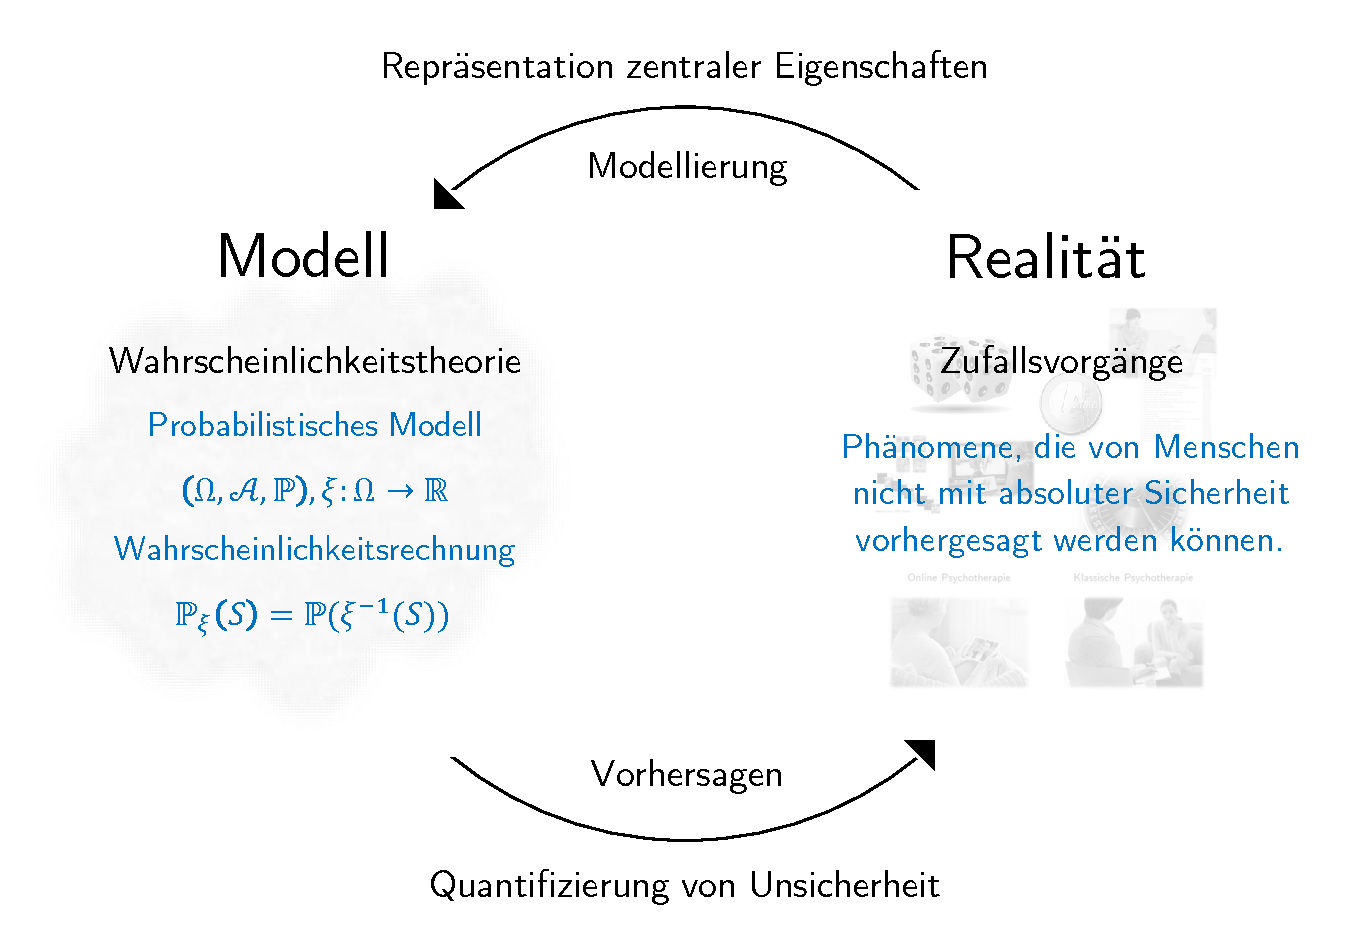
\includegraphics[width=0.85\linewidth]{6_Abbildungen/wtfi_6_wahrscheinlichkeitstheorie_modell} \end{center}
\end{frame}

\begin{frame}{}
\protect\hypertarget{section-4}{}
\begin{center}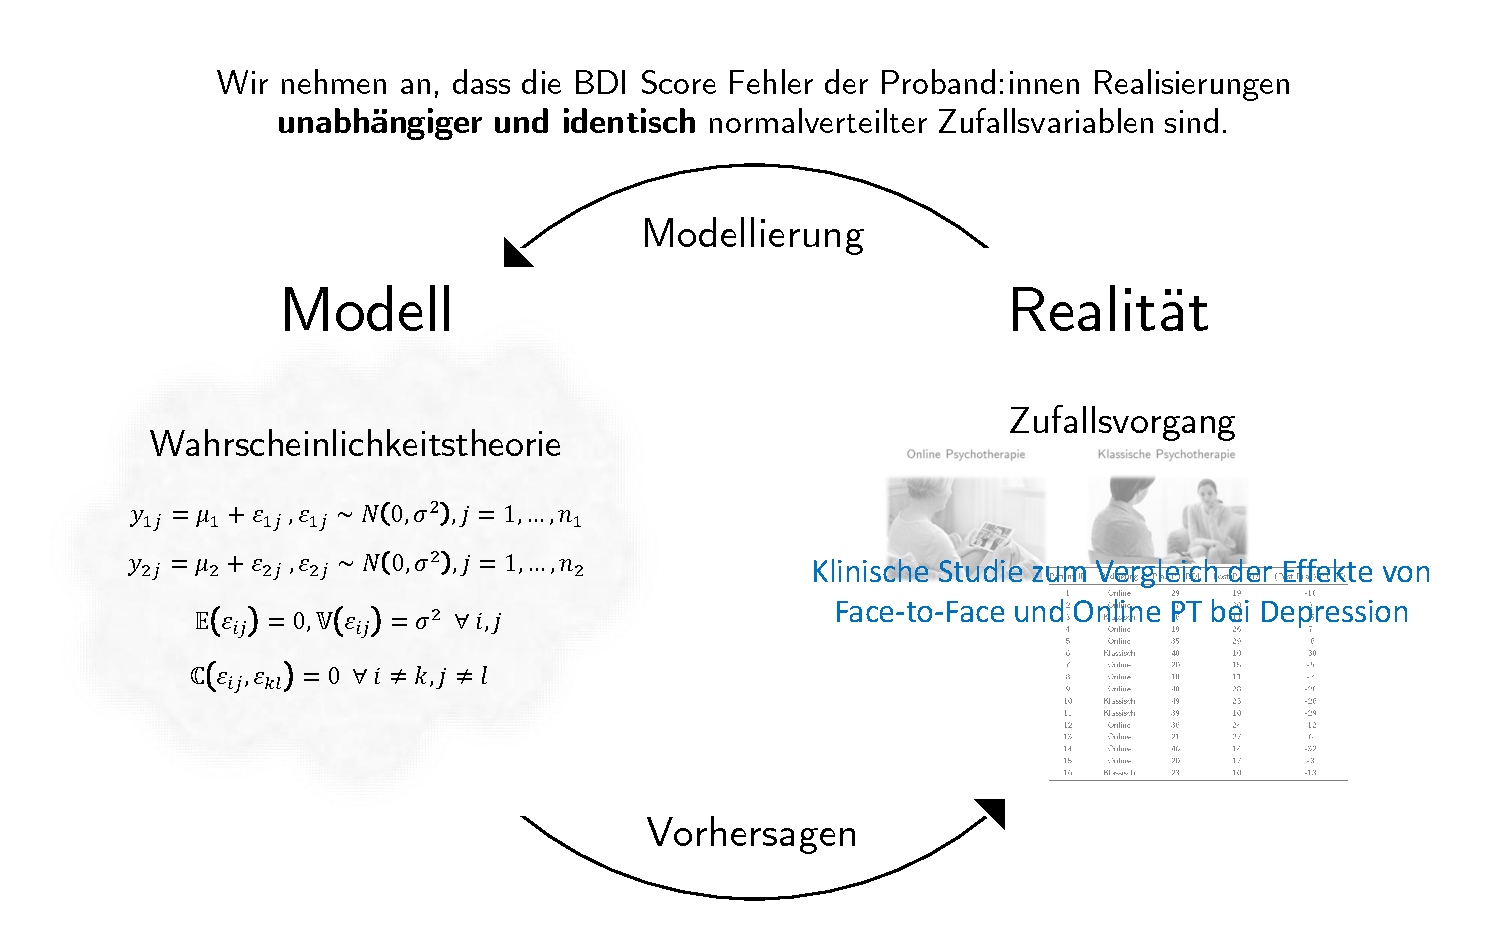
\includegraphics[width=1\linewidth]{6_Abbildungen/wtfi_6_wahrscheinlichkeitstheorie_modell_beispiel} \end{center}
\end{frame}

\begin{frame}{}
\protect\hypertarget{section-5}{}
\setstretch{2.5}
\large
\vfill

Erwartungswert

Varianz und Standardabweichung

Stichprobenmittel, Stichprobenvarianz, Stichprobenstandardabweichung

Kovarianz und Korrelation

Selbstkontrollfragen \vfill
\end{frame}

\begin{frame}{}
\protect\hypertarget{section-6}{}
\setstretch{2.5}
\large
\vfill

\textbf{Erwartungswert}

Varianz und Standardabweichung

Stichprobenmittel, Stichprobenvarianz, Stichprobenstandardabweichung

Kovarianz und Korrelation

Selbstkontrollfragen \vfill
\end{frame}

\begin{frame}{Erwartungswert}
\protect\hypertarget{erwartungswert}{}
\small
\begin{definition}[Erwartungswert]
\justifying
$(\Omega, \mathcal{A},\mathbb{P})$ sei ein Wahrscheinlichkeitsraum und $\xi$
sei eine  Zufallsvariable. Dann ist der \textit{Erwartungswert von $\xi$} definiert als
\begin{itemize}
\item 
$\mathbb{E}(\xi)
:=
\sum_{x \in \mathcal{X}} x\,p_\xi(x)$,
wenn $\xi : \Omega \to \mathcal{X}$ diskret mit WMF $p_\xi$ und Ergebnisraum $\mathcal{X}$ ist,
\item
$\mathbb{E}(\xi)
:=
\intinf x \,p_\xi(x)\,dx$,
wenn $\xi : \Omega \to \mathbb{R}$ kontinuierlich mit WDF $p_\xi$ ist.
\end{itemize}
Der Erwartungswert einer Zufallsvariable heißt \textit{existent}, wenn er endlich ist.
\end{definition}

Bemerkungen

\begin{itemize}
\tightlist
\item
  Der Erwartungswert ist eine skalare Zusammenfassung einer Verteilung.
\item
  Intuitiv ist \(\mathbb{E}(\xi) \approx \frac{1}{n}\sum_{i=1}^n \xi_i\)
  für eine große Zahl \(n\) von Kopien \(\xi_i\) von \(\xi\).
\end{itemize}
\end{frame}

\begin{frame}{Erwartungswert}
\protect\hypertarget{erwartungswert-1}{}
Beispiel (Erwartungswert einer Bernoulli Zufallsvariable) \vspace{2mm}

\small

Es sei \(\xi \sim \mbox{Bern}(\mu)\). Dann gilt
\(\mathbb{E}(\xi) = \mu\). \vspace{5mm}

\underline{Beweis} \vspace{1mm}

\(\xi\) ist diskret mit \(\mathcal{X} = \{0,1\}\). Also gilt
\begin{align}
\begin{split}
\mathbb{E}(\xi)
& = \sum_{x \in \{0,1\}} x\,\mbox{Bern}(x;\mu) \\
& = 0\cdot \mu^0 (1 - \mu)^{1-0} + 1\cdot \mu^1 (1 - \mu)^{1-1} \\
& = 1\cdot \mu^1 (1 - \mu)^{0} \\
& = \mu.
\end{split}
\end{align} \(\hfill \Box\)
\end{frame}

\begin{frame}{Erwartungswert}
\protect\hypertarget{erwartungswert-2}{}
Beispiel (Erwartungswert einer normalverteilten Zufallsvariable)
\vspace{2mm}

\small

Es sei \(\xi \sim N(\mu,\sigma^2)\). Dann gilt
\(\mathbb{E}(\xi) = \mu\).

\vspace{2mm}

\footnotesize

\underline{Beweis} \vspace{1mm}

Wir halten zunächst ohne Beweis fest, dass \begin{equation}
\intinf \exp(-x^2)\,dx = \sqrt{\pi}.
\end{equation} Mit der Definition des Erwartungswerts für
kontinuierliche Zufallsvariablen gilt \begin{equation}
\mathbb{E}(\xi)
= \intinf x \frac{1}{\sqrt{2\pi\sigma^2}}\exp\left(-\frac{1}{2\sigma^2}(x - \mu)^2\right) \,dx.
\end{equation} Mit der Substitutionsregel \begin{equation}
\int_{g(a)}^{g(b)} f(x)\,dx = \int_a^b f(g(x))g'(x)\,dx
\end{equation} und der Definition von \begin{equation}
g : \mathbb{R} \to \mathbb{R}, x \mapsto g(x) := \sqrt{2\sigma^2}x + \mu
\mbox{ with } g'(x) = \sqrt{2\sigma^2},
\end{equation} gilt dann
\end{frame}

\begin{frame}{Erwartungswert}
\protect\hypertarget{erwartungswert-3}{}
\footnotesize

\begin{align}
\begin{split}
\mathbb{E}(\xi)
& = \frac{1}{\sqrt{2\pi\sigma^2}}
\intinf x
\exp\left(-\frac{1}{2\sigma^2}(x - \mu)^2\right) \,dx \\
& = \frac{1}{\sqrt{2\pi\sigma^2}}
\intinf (\sqrt{2\sigma^2}x + \mu)
\exp\left(-\frac{1}{2\sigma^2}\left(\left(\sqrt{2\sigma^2}x + \mu \right) - \mu\right)^2\right)
\sqrt{2\sigma^2}\,dx \\
& = \frac{\sqrt{2\sigma^2}}{\sqrt{2\pi\sigma^2}}
\intinf (\sqrt{2\sigma^2}x + \mu)
\exp\left(-x^2\right) \,dx \\
& = \frac{1}{\sqrt{\pi}}
\left(\sqrt{2\sigma^2} \intinf x \exp\left(-x^2\right) \,dx
      + \mu \intinf \exp\left(-x^2\right) \,dx \right) \\
& = \frac{1}{\sqrt{\pi}}
\left(\sqrt{2\sigma^2} \intinf x \exp\left(-x^2\right) \,dx
      + \mu \sqrt{\pi} \right)
\end{split}
\end{align} Eine Stammfunktion von \(x \exp\left(-x^2\right)\) ist
\(-\frac{1}{2}\exp(-x^2)\). Mit \begin{equation}
\lim_{x \to -\infty} \exp(-x^2) = 0 \mbox{ und } \lim_{x \to \infty}\exp(-x^2) = 0
\end{equation} verschwindet der Integralterm und wir erhalten
\begin{align}
\mathbb{E}(\xi)
= \frac{1}{\sqrt{\pi}}\left(\mu \sqrt{\pi}\right)
= \mu.
\end{align} \(\hfill\Box\)
\end{frame}

\begin{frame}{Erwartungswert}
\protect\hypertarget{erwartungswert-4}{}
\small
\begin{theorem}[Eigenschaften des Erwartungswerts]
\normalfont
\justifying
\begin{itemize}
\item[(1)] (Linear-affine Transformation) Für eine Zufallsvariable $\xi$ und $a,b\in \mathbb{R}$ gilt
\begin{equation}
\mathbb{E}(a\xi + b) = a\mathbb{E}(\xi) + b.
\end{equation}
\item[(2)] (Linearkombination) Für Zufallsvariablen $\xi_1,...,\xi_n$ und $a_1,...,a_n \in \mathbb{R}$ gilt
\begin{equation}
\mathbb{E}\left(\sum_{i=1}^n a_i\xi_i \right) = \sum_{i = 1}^n a_i \mathbb{E}(\xi_i).
\end{equation}
\item [(3)] (Faktorisierung bei Unabhängigkeit) Für unabhängige Zufallsvariablen $\xi_1,...,\xi_n$ gilt
\begin{equation}
\mathbb{E}\left(\prod_{i=1}^n \xi_i \right) = \prod_{i = 1}^n \mathbb{E}(\xi_i).
\end{equation}
\end{itemize}
\end{theorem}

\footnotesize

Bemerkung

\begin{itemize}
\tightlist
\item
  Die genannten Eigenschaften sind oft nützlich zur Berechnung von
  Erwartungswerten.
\end{itemize}
\end{frame}

\begin{frame}{Erwartungswert}
\protect\hypertarget{erwartungswert-5}{}
\footnotesize

\underline{Beweis} \vspace{2mm}

Eigenschaft (1) folgt aus den Linearitätseigenschaften von Summen und
Integralen. Wir betrachten nur den Fall einer kontinuierlichen
Zufallsvariable \(\xi\) mit WDF \(p_\xi\) genauer und definieren
zunächst \(\ups := a\xi + b\). Dann gilt

\begin{align}
\begin{split}
\mathbb{E}(\ups)
& = \mathbb{E}(a\xi + b)                                        \\
& = \intinf (ax + b)p_\xi(x) \,dx                               \\
& = \intinf  axp_\xi(x)  + b p_\xi(x) \,dx                      \\
& = a\intinf xp_\xi(x) \,dx + b \intinf p_\xi(x) \,dx           \\
& = a\mathbb{E}(\xi) + b.
\end{split}
\end{align}
\end{frame}

\begin{frame}{Erwartungswert}
\protect\hypertarget{erwartungswert-6}{}
\footnotesize

\underline{Beweis (fortgeführt)} \vspace{2mm}

Eigenschaft (2) folgt gleichfalls aus den Linearitätseigenschaften von
Summen und Integralen. Wir betrachten nur den Fall von zwei
kontinuierlichen Zufallsvariablen \(\xi_1\) und \(\xi_2\) mit bivariater
WDF \(p_{\xi_1,\xi_2}\) genauer. In diesem Fall gilt \begin{align}
\begin{split}
& \mathbb{E}\left(\sum_{i=1}^2 a_i\xi_i\right)  \\
& = \mathbb{E}(a_1\xi_1 + a_2\xi_2) \\
& = \iint_{\mathbb{R}^2} (a_1x_1 + a_2x_2)p_{\xi_1,\xi_2}(x_1,x_2)\,dx_1\,dx_2  \\
& = \iint_{\mathbb{R}^2} a_1x_1 p_{\xi_1,\xi_2}(x_1,x_2)
                                   + a_2x_2 p_{\xi_1,\xi_2}(x_1,x_2)\,dx_1\,dx_2            \\
& =  a_1\iint_{\mathbb{R}^2} x_1 p_{\xi_1,\xi_2}(x_1,x_2) \,dx_1\,dx_2
  +  a_2\iint_{\mathbb{R}^2} x_2 p_{\xi_1,\xi_2}(x_1,x_2)\,dx_1\,dx_2           \\
\end{split}
\end{align}
\end{frame}

\begin{frame}{Erwartungswert}
\protect\hypertarget{erwartungswert-7}{}
\footnotesize

\underline{Beweis (fortgeführt)} \vspace{2mm}

\begin{align}
\begin{split} 
& =  a_1\intinf x_1 \left(\intinf p_{\xi_1,\xi_2}(x_1,x_2) \,dx_2 \right)\,dx_1
  +  a_2\intinf x_2 \left(\intinf p_{\xi_1,\xi_2}(x_1,x_2) \,dx_1 \right) \,dx_2 \\
& =  a_1\intinf x_1 p_{\xi_1}(x_1) \,dx_1
  +  a_2\intinf x_2 p_{\xi_2}(x_2) \,dx_2 \\
& =  a_1 \mathbb{E}(\xi_1) +  a_2\mathbb{E}(\xi_2) \\
& = \sum_{i=1}^2 a_i \mathbb{E}(\xi_i).
\end{split}
\end{align} Ein Induktionsargument erlaubt dann die Generalisierung vom
bivariaten zum \(n\)-variaten Fall.
\end{frame}

\begin{frame}{Erwartungswert}
\protect\hypertarget{erwartungswert-8}{}
\footnotesize

\underline{Beweis (fortgeführt)}

Zu Eigenschaft (3) betrachten wir den Fall von \(n\) kontinuierlichen
Zufallsvariablen mit gemeinsamer WDF \(p_{\xi_1,...,\xi_n}\). Weil als
\(\xi_1,...,\xi_n\) unabhängig vorausgesetzt sind, gilt \begin{equation}
p_{\xi_1,...,\xi_n}(x_1,...,x_n) = \prod_{i=1}^n p_{\xi_i}(x_i).
\end{equation} Weiterhin gilt also \begin{align}
\begin{split}
\mathbb{E}\left(\prod_{i=1}^n x_i\right)
& = \intinf\cdots\intinf \left(\prod_{i=1}^n x_i\right)
        p_{\xi_1,...,\xi_n}(x_1,...,x_n) \,dx_1...\,dx_n    \\
& = \intinf\cdots\intinf  \prod_{i=1}^n x_i
         \prod_{i=1}^n p_{\xi_i}(x_i)\,dx_1...\,dx_n    \\
& = \intinf\cdots \intinf  \prod_{i=1}^n x_i p_{\xi_i}(x_i) \,dx_1...\,dx_n \\
& = \prod_{i=1}^n \intinf x_i p_{\xi_i}(x_i) \,dx_i 
 = \prod_{i=1}^n \mathbb{E}(\xi_i).
\end{split}
\end{align} \(\hfill \Box\)
\end{frame}

\begin{frame}{}
\protect\hypertarget{section-7}{}
\setstretch{2.5}
\large
\vfill

Erwartungswert

\textbf{Varianz und Standardabweichung}

Stichprobenmittel, Stichprobenvarianz, Stichprobenstandardabweichung

Kovarianz und Korrelation

Stichprobenkovarianz und Stichprobenkorrelation

Selbstkontrollfragen \vfill
\end{frame}

\begin{frame}{Varianz und Standardabweichung}
\protect\hypertarget{varianz-und-standardabweichung}{}
\small
\begin{definition}[Varianz und Standardabweichung]
\justifying
Es sei $\xi$ eine Zufallsvariable mit Erwartungswert $\mathbb{E}(\xi)$. 
Die \textit{Varianz von $\xi$} ist definiert als
\begin{equation}
\mathbb{V}(\xi) := \mathbb{E}\left((\xi - \mathbb{E}(\xi))^2\right),
\end{equation}
unter der Annahme, dass dieser Erwartungswert existiert. Die 
\textit{Standardabweichung von $\xi$} ist definiert
\begin{equation}
\mathbb{S}(\xi) := \sqrt{\mathbb{V}(\xi)}.
\end{equation}
\end{definition}

Bemerkungen

\begin{itemize}
\tightlist
\item
  Die Varianz misst die Streuung (Breite) einer Verteilung.
\item
  Quadration ist nötig wegen
  \(\mathbb{E}(\xi-\mathbb{E}(\xi)) = \mathbb{E}(\xi) - \mathbb{E}(\xi) = 0\).
\item
  Ein alternatives Maß für die Streuung einer Verteilung ist
  \(\mathbb{E}(|\xi - \mathbb{E}(\xi)|)\).
\item
  Ein weiteres Maß für die Streuung einer Verteilung ist die Entropie
  \(-\mathbb{E}(\ln p_\xi)\).
\end{itemize}
\end{frame}

\begin{frame}{Varianz und Standardabweichung}
\protect\hypertarget{varianz-und-standardabweichung-1}{}
Beispiel (Varianz einer Bernoulli Zufallsvariable) \small

Es sei \(\xi \sim \mbox{Bern}(\mu)\). Dann ist die Varianz von \(\xi\)
gegeben durch \begin{equation}
\mathbb{V}(\xi) = \mu(1-\mu).
\end{equation}

\footnotesize

\underline{Beweis} \vspace{1mm}

\(\xi\) ist eine diskrete Zufallsvariable und es gilt
\(\mathbb{E}(\xi) = \mu\). Also gilt \begin{align}
\begin{split}
\mathbb{V}(\xi)
& = \mathbb{E}\left((\xi - \mu)^2\right) \\
& = \sum_{x \in \{0,1\}} (x - \mu)^2 \mbox{Bern}(x;\mu) \\
& = (0 - \mu)^2 \mu^0(1-\mu)^{1-0}  + (1 - \mu)^2\mu^1(1-\mu)^{1-1}  \\
& = \mu^2 (1-\mu)  + (1 - \mu)^2\mu  \\
& = \left(\mu^2  + (1 - \mu)\mu\right)(1-\mu)  \\
& = \left(\mu^2 + \mu - \mu^2\right)(1 - \mu) \\
& = \mu(1-\mu).
\end{split}
\end{align} \(\hfill \Box\)
\end{frame}

\begin{frame}{Varianz und Standardabweichung}
\protect\hypertarget{varianz-und-standardabweichung-2}{}
\small
\begin{theorem}[Varianzverschiebungssatz]
\normalfont
\justifying
Es sei $\xi$ eine Zufallsvariable. Dann gilt
\begin{equation}
\mathbb{V}(\xi) = \mathbb{E}\left(\xi^2 \right) - \mathbb{E}(\xi)^2.
\end{equation}
\end{theorem}

\footnotesize

\underline{Beweis}

Mit der Definition der Varianz und der Linearität des Erwartungswerts
gilt \begin{align}
\begin{split}
\mathbb{V}(\xi)
& = \mathbb{E}\left((\xi - \mathbb{E}(\xi))^2\right) \\
& = \mathbb{E}\left(\xi^2 - 2\xi\mathbb{E}(\xi) + \mathbb{E}(\xi)^2 \right) \\
& =    \mathbb{E}(\xi^2)
    - 2\mathbb{E}(\xi)\mathbb{E}(\xi)
    + \mathbb{E}\left(\mathbb{E}(\xi)^2\right)   \\
& = \mathbb{E}(\xi^2) - 2\mathbb{E}(\xi)^2 + \mathbb{E}(\xi)^2  \\
& = \mathbb{E}(\xi^2) - \mathbb{E}(\xi)^2.
\end{split}
\end{align} \(\hfill \Box\)

Bemerkung

\begin{itemize}
\tightlist
\item
  Das Theorem ist nützlich, wenn \(\mathbb{E}\left(\xi^2 \right)\) und
  \(\mathbb{E}(\xi)\) leicht zu berechnen sind.
\end{itemize}
\end{frame}

\begin{frame}{Varianz und Standardabweichung}
\protect\hypertarget{varianz-und-standardabweichung-3}{}
\small

Beispiel (Varianz einer normalverteilten Zufallsvariable) \vspace{1mm}

Es sei \(\xi \sim N(\mu,\sigma^2)\). Dann gilt
\(\mathbb{V}(\xi) = \sigma^2\). \vspace{3mm}

\footnotesize

\underline{Beweis} \vspace{1mm}

Wir halten zunächst fest, dass mit dem Varianzverschiebungssatz gilt,
dass \begin{align}\label{eq:var_gauss_1}
\begin{split}
\mathbb{V}(\xi)
= \mathbb{E}(\xi^2) - \mathbb{E}(\xi)^2
= \frac{1}{2\pi\sigma^2}\intinf x^2 \exp\left(-\frac{1}{2\sigma^2}(x-\mu)^2 \right)\,dx - \mu^2
\end{split}
\end{align}

Mit der Substitutionsregel \begin{equation}
\int_{a}^{b} f(g(x))g'(x)\,dx = \int_{g(a)}^{g(b)} f(x)\,dx
\end{equation} und der Definition von \begin{equation}
g:\mathbb{R} \to \mathbb{R}, x \mapsto \sqrt{2\sigma^2}x + \mu,
g(-\infty) := -\infty, g(\infty) := \infty,
\mbox{ with }
g'(x) = \sqrt{2\sigma^2},
\end{equation} kann das Integral auf der rechten Seite von Gleichung
\eqref{eq:var_gauss_1} dann als
\end{frame}

\begin{frame}{Varianz und Standardabweichung}
\protect\hypertarget{varianz-und-standardabweichung-4}{}
\footnotesize
\setstretch{1.2}

\underline{Beweis (fortgeführt)} \begin{align}
\begin{split}
\intinf x^2 \exp & \left(-\frac{1}{2\sigma^2}(x - \mu)^2 \right) \,dx \\
& =
\intinf (\sqrt{2\sigma^2}x + \mu)^2 \exp\left(-\frac{1}{2\sigma^2}((\sqrt{2\sigma^2}x + \mu)-\mu)^2 \right)\sqrt{2\sigma^2}\,dx \\
& =
\sqrt{2\sigma^2}\intinf (\sqrt{2\sigma^2}x + \mu)^2 \exp\left(-\frac{2\sigma^2 x^2}{2\sigma^2} \right)\,dx \\
& =
\sqrt{2\sigma^2}\intinf (\sqrt{2\sigma^2}x + \mu)^2 \exp\left(-x^2\right)\,dx.
\end{split}
\end{align} geschrieben werden. Also gilt

\begin{tiny}
\begin{align*}
\begin{split}
\mathbb{V}(\xi)
& =
\frac{\sqrt{2\sigma^2}}{\sqrt{2\pi\sigma^2}}
\intinf (\sqrt{2\sigma^2}x + \mu)^2 \exp\left(-x^2 \right)\,dx
- \mu^2
\\
&
= \frac{1}{\sqrt{\pi}}
\intinf(\sqrt{2\sigma^2}x)^2 + 2\sqrt{2\sigma^2}x\mu + \mu^2) \exp\left(-x^2 \right)\,dx
- \mu^2
\\
&
= \frac{1}{\sqrt{\pi}}
\left(
        2\sigma^2\intinf x^2 \exp\left(-x^2 \right)\,dx +
        2\sqrt{2\sigma^2}\mu\intinf x\exp\left(-x^2 \right)\,dx +
        \mu^2\intinf \exp\left(-x^2 \right)\,dx
\right)
- \mu^2
\end{split}
\end{align*}
\end{tiny}
\end{frame}

\begin{frame}{Varianz und Standardabweichung}
\protect\hypertarget{varianz-und-standardabweichung-5}{}
\footnotesize

\underline{Beweis (fortgeführt)} \vspace{1mm}

Wir halten weiterhin ohne Beweis fest, dass \begin{equation}
\intinf x \exp(-x^2)\,dx = 0
\mbox{ und }
\intinf \exp(-x^2)\,dx = \sqrt{\pi}.
\end{equation} Es ergibt sich dann \begin{align}
\begin{split}
\mathbb{V}(\xi)
& = \frac{1}{\sqrt{\pi}}
\left(2\sigma^2\intinf x^2 \exp\left(-x^2 \right)\,dx + \mu^2\sqrt{\pi} \right)
- \mu^2
\\
& = \frac{2\sigma^2}{\sqrt{\pi}}
\intinf x^2 \exp\left(-x^2 \right)\,dx
+ \mu^2 - \mu^2
\\
& = \frac{2\sigma^2}{\sqrt{\pi}} \intinf x^2 \exp\left(-x^2 \right)\,dx
\end{split}
\end{align} Mit der partiellen Integrationsregel \begin{equation}
\int_{a}^{b} f'(x)g(x)\,dx =
f(x)g(x)|_{a}^{b} - \int_{a}^{b} f(x)g'(x)\,dx
\end{equation} und der Definition von \begin{equation}
f : \mathbb{R} \to \mathbb{R}, x \mapsto f(x) := \exp(-x^2) \mbox{ with } f'(x) = -2\exp(-x^2)
\end{equation}
\end{frame}

\begin{frame}{Varianz und Standardabweichung}
\protect\hypertarget{varianz-und-standardabweichung-6}{}
\footnotesize

\underline{Beweis (fortgeführt)} \vspace{1mm}

und \begin{equation}
g : \mathbb{R} \to \mathbb{R}, x\mapsto g(x) := -\frac{1}{2}x \mbox{ with } g'(x) = -\frac{1}{2},
\end{equation} so dass \begin{equation}
f'(x)g(x) = -2\exp(-x^2)\left(-\frac{1}{2}x \right) = x^2\exp(-x^2),
\end{equation} gilt, ergibt sich dann \begin{align}
\begin{split}
\mathbb{V}(\xi)
& = \frac{2\sigma^2}{\sqrt{\pi}} \intinf x^2 \exp\left(-x^2 \right)\,dx  \\
& = \frac{2\sigma^2}{\sqrt{\pi}}
\left( -\frac{1}{2}x\exp(-x^2)|_{-\infty}^{\infty}
- \intinf \exp\left(-x^2 \right)\left(-\frac{1}{2} \right)\,dx \right)  \\
& = \frac{2\sigma^2}{\sqrt{\pi}}
\left(
 -\frac{1}{2}x\exp(-x^2)|_{-\infty}^{\infty}
+ \frac{1}{2}\intinf \exp\left(-x^2 \right)\,dx
\right),
\end{split}
\end{align} Aus \(\lim_{x\to \pm \infty} \exp(-x^2) = 0\) schließen wir,
dass der erste Term in den Klammern auf der rechten Seite der obigen
Gleichung gleich \(0\) ist. Schließlich ergibt sich \begin{align}
\begin{split}
\mathbb{V}(\xi)
= \frac{2\sigma^2}{\sqrt{\pi}} \left(\frac{1}{2}\intinf \exp\left(-x^2 \right)\,dx\right)
= \frac{\sigma^2}{\sqrt{\pi}} \sqrt{\pi}
= \sigma^2.
\end{split}
\end{align} \(\hfill\Box\)
\end{frame}

\begin{frame}{Varianz und Standardabweichung}
\protect\hypertarget{varianz-und-standardabweichung-7}{}
\small
\begin{theorem}[Eigenschaften der Varianz]
\normalfont
\justifying
\begin{itemize}
\item[(1)] (Linear-affine Transformation) Für eine Zufallsvariable $\xi$ und 
$a,b\in \mathbb{R}$ gelten
\begin{equation}
\mathbb{V}(a\xi + b) = a^2 \mathbb{V}(\xi)
\mbox{ und }
\mathbb{S}(a\xi + b) = |a|\mathbb{S}(\xi).
\end{equation}
\item [(2)] (Linearkombination bei Unabhängigkeit) Für unabhängige 
Zufallsvariablen $\xi_1,...,\xi_n$ und $a_1,...,a_n \in \mathbb{R}$ gilt
\begin{equation}
\mathbb{V}\left(\sum_{i=1}^n a_i\xi_i\right) = \sum_{i=1}^n a_i^2 \mathbb{V}(\xi_i).
\end{equation}
\end{itemize}
\end{theorem}
\end{frame}

\begin{frame}{Varianz und Standardabweichung}
\protect\hypertarget{varianz-und-standardabweichung-8}{}
\footnotesize

\underline{Beweis} \vspace{1mm}

Um Eigenschaft (1) zu zeigen, definieren wir zunächst
\(\ups := a\xi + b\) und halten fest, dass
\(\mathbb{E}(\ups) = a\mathbb{E}(\xi) + b\). Für die Varianz von
\(\ups\) ergibt sich dann \begin{align}
\begin{split}
\mathbb{V}(\ups)
& = \mathbb{E}\left((\ups - \mathbb{E}(\ups))^2\right)      \\
& = \mathbb{E}\left((a\xi+b-a\mathbb{E}(\xi)-b)^2\right)    \\
& = \mathbb{E}\left((a\xi-a\mathbb{E}(\xi))^2\right)        \\
& = \mathbb{E}\left((a(\xi - \mathbb{E}(\xi))^2\right)      \\
& = \mathbb{E}\left(a^2(\xi - \mathbb{E}(\xi))^2\right)     \\
& = a^2\mathbb{E}\left((\xi - \mathbb{E}(\xi))^2\right)     \\
& = a^2\mathbb{V}(\xi)                                  \\
\end{split}
\end{align} Wurzelziehen ergibt dann das Resultat für die
Standardabweichung. \vspace{1mm}

Für Eigenschaft (2) betrachten wir den Fall zweier unabhängiger
Zufallsvariablen \(\xi_1\) und \(\xi_2\) genauer. Wir halten zunächst
fest, dass in diesem Fall gilt, dass \begin{equation}
\mathbb{E}\left(a_1\xi_1 + a_2\xi_2\right) = a_1\mathbb{E}(\xi_1) + a_2\mathbb{E}(\xi_2).
\end{equation}
\end{frame}

\begin{frame}{Varianz und Standardabweichung}
\protect\hypertarget{varianz-und-standardabweichung-9}{}
\footnotesize
\vspace{2mm}

\underline{Beweis (fortgeführt)}

Es ergibt sich also \begin{align*}
\begin{split}
& \mathbb{V}\left(\sum_{i=1}^2 a_i \xi_i\right)                                                   \\
& = \mathbb{V}(a_1\xi_1 + a_2\xi_2)                                                               \\
& = \mathbb{E}\left((a_1\xi_1 + a_2\xi_2 - \mathbb{E}\left(a_1\xi_1 + a_2\xi_2\right))^2\right)   \\
& = \mathbb{E}\left((a_1\xi_1 + a_2\xi_2 - a_1\mathbb{E}(\xi_1) - a_2\mathbb{E}(\xi_2))^2\right)  \\
& = \mathbb{E}\left((a_1\xi_1 - a_1\mathbb{E}(\xi_1) + a_2\xi_2  - a_2\mathbb{E}(\xi_2))^2\right) \\
& = \mathbb{E}\left(((a_1(\xi_1 - \mathbb{E}(\xi_1)) + (a_2(\xi_2 - \mathbb{E}(\xi_2)))^2\right)  \\
& = \mathbb{E}\left((a_1(\xi_1 - \mathbb{E}(\xi_1)))^2
                   + 2(a_1(\xi_1 - \mathbb{E}(\xi_1))(a_2(\xi_2 - \mathbb{E}(\xi_2))
                   + (a_2(\xi_2 - \mathbb{E}(\xi_2)))^2\right) \\
& = \mathbb{E}\left((a_1^2(\xi_1 - \mathbb{E}(\xi_1))^2
                   + 2a_1a_2(\xi_1 - \mathbb{E}(\xi_1))(\xi_2 - \mathbb{E}(\xi_2))
                   + a_2^2(\xi_2 - \mathbb{E}(\xi_2))^2\right) \\
& = a_1^2\mathbb{E}\left((\xi_1 - \mathbb{E}(\xi_1))^2\right)
   + 2a_1a_2\mathbb{E}\left((\xi_1 - \mathbb{E}(\xi_1))(\xi_2 - \mathbb{E}(\xi_2))\right)
   + a_2^2\mathbb{E}\left((\xi_2 - \mathbb{E}(\xi_2))^2\right) \\
& = a_1^2\mathbb{V}(\xi_1)
   + 2a_1a_2\mathbb{E}\left((\xi_1 - \mathbb{E}(\xi_1))(\xi_2 - \mathbb{E}(\xi_2))\right)
   + a_2^2\mathbb{V}(\xi_2) \\
& = \sum_{i=1}^2 a_i^2\mathbb{V}(\xi_i)
   + 2a_1a_2\mathbb{E}\left((\xi_1 - \mathbb{E}(\xi_1))(\xi_2 - \mathbb{E}(\xi_2))\right).
\end{split}.
\end{align*}
\end{frame}

\begin{frame}{Varianz und Standardabweichung}
\protect\hypertarget{varianz-und-standardabweichung-10}{}
\footnotesize

\underline{Beweis (fortgeführt)} \vspace{2mm}

Weil \(\xi_1\) und \(\xi_2\) unabhängig sind, ergibt sich mit den
Eigenschaften des Erwartungswerts für unabhängige Zufallsvariablen, dass
\begin{align}
\begin{split}
\mathbb{E}\left((\xi_1 - \mathbb{E}(\xi_1))(\xi_2 - \mathbb{E}(\xi_2))\right)
& = \mathbb{E}\left((\xi_1 - \mathbb{E}(\xi_1))\right)
    \mathbb{E}\left((\xi_2 - \mathbb{E}(\xi_2))\right) \\
& = (\mathbb{E}(\xi_1) - \mathbb{E}(\xi_1))
    (\mathbb{E}(\xi_2) - \mathbb{E}(\xi_2)) \\
& = 0
\end{split}
\end{align} ist. Damit folgt also \begin{equation}
\mathbb{V}\left(\sum_{i=1}^2 a_i \xi_i\right)
=  \sum_{i=1}^2 a_i^2\mathbb{V}(\xi_i).
\end{equation} Ein Induktionsargument erlaubt dann die Generalisierung
vom bivariaten zum \(n\)-variaten Fall.

\(\hfill\Box\)
\end{frame}

\begin{frame}{}
\protect\hypertarget{section-8}{}
\setstretch{2.5}
\large
\vfill

Erwartungswert

Varianz und Standardabweichung

\normalsize

\textbf{Stichprobenmittel, Stichprobenvarianz,
Stichprobenstandardabweichung}

\large

Kovarianz und Korrelation

Selbstkontrollfragen \vfill
\end{frame}

\begin{frame}{Stichprobenmittel, Stichprobenvarianz,
Stichprobenstandardabweichung}
\protect\hypertarget{stichprobenmittel-stichprobenvarianz-stichprobenstandardabweichung}{}
\setstretch{1.1}
\footnotesize
\begin{definition}[Stichprobenmittel, -varianz, -standardabweichung]
$\xi_1,...,\xi_n$ seien Zufallsvariablen. Dann nennt man $\xi_1,...,\xi_n$ auch eine \textit{Stichprobe}.
\begin{itemize}
\item Das \textit{Stichprobenmittel} von $\xi_1,...,\xi_n$ ist definiert als der arithmetische Mittelwert
\begin{equation}
\bar{\xi}_n := \frac{1}{n}\sum_{i=1}^n \xi_i.
\end{equation}
\item Die \textit{Stichprobenvarianz} von $\xi_1,...,\xi_n$ ist definiert als
\begin{equation}
S_n^2 := \frac{1}{n-1}\sum_{i=1}^n (\xi_i - \bar{\xi}_n)^2.
\end{equation}
\item  Die \textit{Stichprobenstandardabweichung} ist definiert als
\begin{equation}
S_n := \sqrt{S_n^2}.
\end{equation}
\end{itemize}
\end{definition}
\vspace{-2mm}
\setstretch{1.3}
\footnotesize

Bemerkungen

\begin{itemize}
\tightlist
\item
  \(\mathbb{E}(\xi),\mathbb{V}(\xi)\), und \(\mathbb{S}(\xi)\) sind
  Kennzahlen einer Zufallsvariable \(\xi\).
\item
  \(\bar{\xi}_n, S_n^2\), und \(S_n\) sind Kennzahlen einer Stichprobe
  \(\xi_1,...,\xi_n\).
\item
  \(\bar{\xi}_n, S_n^2\), und \(S_n\) sind Zufallsvariablen, ihre
  Realisationen werden mit \(\bar{x}_n, s_n^2,\) und \(s_n\) bezeichnet.
\end{itemize}
\end{frame}

\begin{frame}{Stichprobenmittel, Stichprobenvarianz,
Stichprobenstandardabweichung}
\protect\hypertarget{stichprobenmittel-stichprobenvarianz-stichprobenstandardabweichung-1}{}
Beispiel (Stichprobenmittel, Stichprobenvarianz,
Stichprobenstandardabweichung) \vspace{2mm}

\footnotesize

\begin{itemize}
\tightlist
\item
  Es seien \(\xi_1,...,\xi_{10} \sim N(1,2)\).
\item
  Wir nehmen die folgenden Realisationen an
\end{itemize}

\begin{table}[h]
\begin{center}
\begin{tabular}{ccccccccccc}
   $x_1$
&  $x_2$
&  $x_3$
&  $x_4$
&  $x_5$
&  $x_6$
&  $x_7$
&  $x_8$
&  $x_9$
&  $x_{10}$ \\\hline
   0.54
&  1.01
& -3.28
&  0.35
&  2.75
& -0.51
&  2.32
&  1.49
&  0.96
&  1.25
\end{tabular}
\end{center}
\end{table}

\begin{itemize}
\tightlist
\item
  Die Stichprobenmittelrealisation ist \begin{equation}
  \bar{x}_{10}
  = \frac{1}{10}\sum_{i = 1}^{10}x_i
  = \frac{6.88}{10}
  = 0.68.
  \end{equation}
\item
  Die Stichprobenvarianzrealisation ist \begin{equation}
  s_{10}^2
  = \frac{1}{9}\sum_{i=1}^{10} (x_i - \bar{x}_{10})^2
  = \frac{1}{9}\sum_{i=1}^{10} (x_i - 0.68)^2
  = \frac{25.37}{9}
  = 2.82.
  \end{equation}
\item
  Die Stichprobenstandardabweichungrealisation ist \begin{equation}
  s_{10} = \sqrt{s_{10}^2} = \sqrt{2.82} = 1.68.
  \end{equation}
\end{itemize}
\end{frame}

\begin{frame}{}
\protect\hypertarget{section-9}{}
\setstretch{2.5}
\large
\vfill

Erwartungswert

Varianz und Standardabweichung

Stichprobenmittel, Stichprobenvarianz, Stichprobenstandardabweichung

\textbf{Kovarianz und Korrelation}

Selbstkontrollfragen \vfill
\end{frame}

\begin{frame}{Kovarianz und Korrelation}
\protect\hypertarget{kovarianz-und-korrelation}{}
\small
\begin{definition}[Kovarianz und Korrelation]
\justifying
Die \textit{Kovarianz} zweier Zufallsvariablen $\xi$ und $\ups$ ist definiert als
\begin{equation}
\mathbb{C}(\xi,\ups) :=
\mathbb{E}\left(\left(\xi - \mathbb{E}(\xi) \right)\left(\ups - \mathbb{E}(\ups)\right)\right).
\end{equation}
Die \textit{Korrelation} zweier Zufallsvariablen $\xi$ und $\ups$ ist definiert als
\begin{equation}
\rho(\xi,\ups)
:= \frac{\mathbb{C}(\xi,\ups)}{\sqrt{\mathbb{V}(\xi)}\sqrt{\mathbb{V}(\ups)}}
 = \frac{\mathbb{C}(\xi,\ups)}{\mathbb{S}(\xi){\mathbb{S}(\ups)}}.
\end{equation}
\end{definition}

\footnotesize

Bemerkungen

\begin{itemize}
\tightlist
\item
  Die Kovarianz von \(\xi\) mit sich selbst ist die Varianz von \(\xi\),
  \begin{equation}
  \mathbb{C}(\xi,\xi) =
  \mathbb{E}\left(\left(\xi - \mathbb{E}(\xi) \right)^2\right) =
  \mathbb{V}(\xi).
  \end{equation}
\item
  \(\rho(\xi,\ups)\) wird auch \textit{Korrelationskoeffizient} von
  \(\xi\) und \(\ups\) genannt.
\item
  Wenn \(\rho(\xi,\ups) = 0\) ist, werden \(\xi\) und \(\ups\)
  \textit{unkorreliert} genannt.
\item
  Wir zeigen später mit der Cauchy-Schwarz Ungleichung, dass
  \(-1 \le \rho(\xi,\ups) \le 1\).
\end{itemize}
\end{frame}

\begin{frame}{Kovarianz und Korrelation}
\protect\hypertarget{kovarianz-und-korrelation-1}{}
Beispiel (Kovarianz und Korrelation zweier diskreter Zufallsvariablen)
\vspace{1mm}

\footnotesize

Es sei \(\xi := (\xi_1,\xi_2)\) ein Zufallsvektor mit WMF
\(p_{\xi_1,\xi_2}\) definiert durch

\center
\renewcommand{\arraystretch}{1.4}
\begin{tabular}{c|ccc|c}
$p_{\xi_1,\xi_2}(x_1,x_2)$  &   $x_2 = 1$   &   $x_2 = 2$   &   $x_2 = 3$   &   $p_{\xi_1}(x_1)$        \\\hline
$x_1 = 1$               &   $0.10$      &   $0.05$      &   $0.15$      &   $0.30$              \\
$x_1 = 2$               &   $0.60$      &   $0.05$      &   $0.05$      &   $0.70$              \\\hline
$p_{\xi_2}(x_2)$    &   $0.70$      &   $0.10$      &   $0.20$      &                       \\
\end{tabular}
\vspace{1mm}

\flushleft

\(\xi_1\), \(\xi_2\) sind also zwei Zufallsvariablen mit einer
definierten bivariaten Verteilung. Um \(\mathbb{C}(\xi_1,\xi_2)\) und
\(\rho(\xi_1,\xi_2)\) zu berechnen, halten wir zunächst fest, dass
\begin{equation}
\mathbb{E}(\xi_1) = \sum_{x_1=1}^2 x_1 p_{\xi_1}(x_1) = 1\cdot 0.3 + 2\cdot 0.7 = 1.7
\end{equation} und \begin{equation}
\mathbb{E}(\xi_2) = \sum_{x_2=1}^3 x_2 p_{\xi_2}(x_2) = 1\cdot 0.7 + 2\cdot 0.1 + 3\cdot 0.2 = 1.5.
\end{equation} Mit der Definition der Kovarianz von \(\xi_1\) und
\(\xi_2\), gilt dann
\end{frame}

\begin{frame}{Kovarianz und Korrelation}
\protect\hypertarget{kovarianz-und-korrelation-2}{}
\setstretch{1.2}
\begin{tiny}
\begin{align*}
\begin{split}
& \mathbb{C}(\xi_1,\xi_2)                                                                                       \\
& = \mathbb{E}((\xi_1 - \mathbb{E}(\xi_1))(\xi_2 - \mathbb{E}(\xi_2)))                                              \\
& = \sum_{x_1 = 1}^2 \sum_{x_2 = 1}^3 (x_1 - \mathbb{E}(\xi_1))(x_2 - \mathbb{E}(\xi_2))p_{\xi_1,\xi_2}(x_1,x_2)    \\
& = \sum_{x_1 = 1}^2 \sum_{x_2 = 1}^3 (x_1 - 1.7)(x_2 - 1.5)p_{\xi_1,\xi_2}(x_1,x_2)                            \\
& = \sum_{x_1 = 1}^2    (x_1 - 1.7)(1 - 1.5)p_{\xi_1,\xi_2}(x_1,1)                                              \\
&   \quad\quad\quad  +  (x_1 - 1.7)(2 - 1.5)p_{\xi_1,\xi_2}(x_1,2)                                              \\
&   \quad\quad\quad  +  (x_1 - 1.7)(3 - 1.5)p_{\xi_1,\xi_2}(x_1,3)                                              \\
& = \quad       (1 - 1.7)(1 - 1.5)p_{\xi_1,\xi_2}(1,1)
            +   (1 - 1.7)(2 - 1.5)p_{\xi_1,\xi_2}(1,2)
            +   (1 - 1.7)(3 - 1.5)p_{\xi_1,\xi_2}(1,3)                                                          \\
& \quad\,   +   (2 - 1.7)(1 - 1.5)p_{\xi_1,\xi_2}(2,1)
            +   (2 - 1.7)(2 - 1.5)p_{\xi_1,\xi_2}(2,2)
            +   (2 - 1.7)(3 - 1.5)p_{\xi_1,\xi_2}(2,3)                                                          \\
& = \quad       (-0.7)\cdot (-0.5) \cdot 0.10   \quad\quad\quad\quad\quad\quad
            +   (-0.7)\cdot   0.5  \cdot 0.05   \quad\quad\quad\quad\quad\quad\quad\quad
            +   (-0.7)\cdot   1.5  \cdot 0.15                                                               \\
& \quad\,   +   0.3   \cdot (-0.5) \cdot 0.60   \quad\quad\quad\quad\quad\quad\quad\quad
            +   0.3   \cdot   0.5  \cdot 0.05   \quad\quad\quad\quad\quad\quad\quad\quad\quad\quad
            +   0.3   \cdot   1.5  \cdot 0.05                                                               \\
& = \,    0.035
        - 0.0175
        - 0.1575
        - 0.09
        + 0.0075
        + 0.0225\\
& = - 0.2.
\end{split}
\end{align*}
\end{tiny}
\end{frame}

\begin{frame}{Kovarianz und Korrelation}
\protect\hypertarget{kovarianz-und-korrelation-3}{}
\begin{theorem}[Kovarianzverschiebungssatz]
\normalfont
\justifying
$\xi$ und $\ups$ seien Zufallsvariablen. Dann gilt
\begin{equation}
\mathbb{C}(\xi,\ups) = \mathbb{E}(\xi\ups) - \mathbb{E}(\xi)\mathbb{E}(\ups).
\end{equation}
\end{theorem}

\footnotesize

\underline{Beweis}

Mit der Definition der Kovarianz gilt \begin{align}
\begin{split}
\mathbb{C}(\xi,\ups)
& = \mathbb{E}\left((\xi - \mathbb{E}(\xi))(\ups - \mathbb{E}(\ups))\right)                                             \\
& = \mathbb{E}\left(\xi\ups - \xi\mathbb{E}(\ups) - \mathbb{E}(\xi)\ups  + \mathbb{E}(\xi) \mathbb{E}(\ups)\right)          \\
& = \mathbb{E}(\xi\ups) - \mathbb{E}(\xi)\mathbb{E}(\ups) - \mathbb{E}(\xi)\mathbb{E}(\ups) + \mathbb{E}(\xi) \mathbb{E}(\ups)  \\
& = \mathbb{E}(\xi\ups) - \mathbb{E}(\xi)\mathbb{E}(\ups).
\end{split}
\end{align} \(\hfill \Box\)

\footnotesize

Bemerkungen

\justifying

\begin{itemize}
\tightlist
\item
  Das Theorem ist nützlich, wenn
  \(\mathbb{E}(\xi\ups),\mathbb{E}(\xi)\), und \(\mathbb{E}(\ups)\)
  leicht zu berechnen sind.
\item
  Für \(\ups = \xi\) erhalten wir
  \(\mathbb{V}(\xi) = \mathbb{E}(\xi^2) - \mathbb{E}(\xi)^2\).
\end{itemize}
\end{frame}

\begin{frame}{Kovarianz und Korrelation}
\protect\hypertarget{kovarianz-und-korrelation-4}{}
\small
\begin{theorem}[Varianzen von Summen und Differenzen von Zufallsvariablen]
\normalfont
\justifying
$\xi$ und $\ups$ seien zwei Zufallsvariablen und es seien $a,b,c \in \mathbb{R}$. Dann gilt
\begin{equation}
\mathbb{V}(a\xi + b\ups + c) = a^2\mathbb{V}(\xi) + b^2\mathbb{V}(\ups) + 2ab\mathbb{C}(\xi,\ups).
\end{equation}

Speziell gelten
\begin{equation}
\mathbb{V}(\xi+\ups) = \mathbb{V}(\xi) + \mathbb{V}(\ups) + 2 \mathbb{C}(\xi,\ups)
\end{equation}
und
\begin{equation}
\mathbb{V}(\xi-\ups) = \mathbb{V}(\xi) + \mathbb{V}(\ups) - 2 \mathbb{C}(\xi,\ups)
\end{equation}
\end{theorem}

\footnotesize

Bemerkungen

\begin{itemize}
\tightlist
\item
  Varianzen von Zufallsvariablen addieren sich nicht einfach.
\item
  Die Varianz der Summe zweier Zufallsvariablen hängt von ihrer
  Kovarianz ab.
\end{itemize}
\end{frame}

\begin{frame}{Kovarianz und Korrelation}
\protect\hypertarget{kovarianz-und-korrelation-5}{}
\footnotesize

\underline{Beweis} \vspace{2mm}

Wir halten zunächst fest, dass \begin{equation}
\mathbb{E}(a\xi + b\ups + c) = a\mathbb{E}(\xi) + b\mathbb{E}(\ups) + c.
\end{equation}

Es ergibt sich also \begin{align}
\begin{split}
& \mathbb{V}(a\xi + b\ups + c)                                                              \\
& = \mathbb{E}\left((a\xi + b\ups + c - a\mathbb{E}(\xi) - b\mathbb{E}(\ups) - c)^2\right)  \\
& = \mathbb{E}\left((a(\xi  - \mathbb{E}(\xi)) + b(\ups  - \mathbb{E}(\ups)))^2\right)      \\
& = \mathbb{E}\left(a^2(\xi - \mathbb{E}(\xi))^2
                  + 2ab(\xi - \mathbb{E}(\xi))(\ups - \mathbb{E}(\ups)))
                  + b^2(\ups - \mathbb{E}(\ups))^2
                  \right)               \\
& = a^2\mathbb{E}\left((\xi - \mathbb{E}(\xi))^2\right)
  + b^2\mathbb{E}\left((\ups - \mathbb{E}(\ups))^2\right)
  + 2ab\mathbb{E}\left((\xi - \mathbb{E}(\xi))(\ups - \mathbb{E}(\ups)))\right)                 \\
& = a^2\mathbb{V}(\xi)+ b^2\mathbb{V}(\ups) + 2ab\mathbb{C}(\xi,\ups)
\end{split}
\end{align}

Die Spezialfälle folgen dann direkt mit \(a := b := 1\) und
\(a := 1, b := -1\), respektive.

\(\hfill \Box\)
\end{frame}

\begin{frame}{Kovarianz und Korrelation}
\protect\hypertarget{kovarianz-und-korrelation-6}{}
\small
\begin{theorem}[Korrelation und Unabhängigkeit]
\justifying
\normalfont
$\xi$ und $\ups$ seien zwei Zufallsvariablen. Wenn $\xi$ und $\ups$ unabhängig sind, 
dann ist $\mathbb{C}(\xi,\ups) = 0$ und $\xi$ und $\ups$ sind unkorreliert. Ist dagegen
$\mathbb{C}(\xi,\ups) = 0$ und sind $\xi$ und $\ups$ somit unkorreliert, dann sind $\xi$ 
und $\ups$ nicht notwendigerweise unabhängig.
\end{theorem}

\footnotesize

\underline{Beweis} \vspace{1mm}

Wir zeigen zunächst, dass aus der Unabhängigkeit von \(\xi\) und
\(\ups\) \(\mathbb{C}(\xi,\ups) = 0\) folgt. Hierzu halten wir zunächst
fest, dass für unabhängige Zufallsvariablen gilt, dass \begin{equation}
\mathbb{E}(\xi\ups) = \mathbb{E}(\xi)\mathbb{E}(\ups).
\end{equation} Mit dem Kovarianzverschiebungssatz folgt dann
\begin{equation}
\mathbb{C}(\xi,\ups)
= \mathbb{E}(\xi\ups) - \mathbb{E}(\xi)\mathbb{E}(\ups)
= \mathbb{E}(\xi)\mathbb{E}(\ups) - \mathbb{E}(\xi)\mathbb{E}(\ups)
= 0.
\end{equation} Mit der Definition des Korrelationskoeffizienten folgt
dann unmittelbar, dass \(\rho(\xi,\ups) = 0\) und \(\xi\) und \(\ups\)
somit unkorreliert sind.
\end{frame}

\begin{frame}{Kovarianz und Korrelation}
\protect\hypertarget{kovarianz-und-korrelation-7}{}
\footnotesize

\underline{Beweis (fortgeführt)} \vspace{2mm}

Wir zeigen nun durch Angabe eines Beispiels, dass die Kovarianz von
abhängigen Zufallsvariablen \(\xi\) und \(\ups\) null sein kann.

Zu diesem Zweck betrachten wir den Fall zweier diskreter
Zufallsvariablen \(\xi\) und \(\ups\) mit Ergebnisräumen
\(\mathcal{X} = \{-1,0,1\}\) und \(\mathcal{\ups} = \{0,1\}\),
marginaler WMF von \(\xi\) gegeben durch \(p_\xi(x) := 1/3\) für
\(x \in \mathcal{X}\) und der Definition \(\ups := \xi^2\).

Wir halten dann zunächst fest, dass \begin{equation}
\mathbb{E}(\xi)
= \sum_{x \in \mathcal{X}} x p_\xi(x)
= -1 \cdot \frac{1}{3} + 0\cdot \frac{1}{3} + 1\cdot\frac{1}{3}
= 0
\end{equation} und \begin{equation}
\mathbb{E}(\xi\ups)
= \mathbb{E}(\xi\xi^2)
= \mathbb{E}(\xi^3)
= \sum_{x \in \mathcal{X}} x^3 p_\xi(x)
= -1^3 \cdot \frac{1}{3} + 0^3\cdot \frac{1}{3} + 1^3\cdot\frac{1}{3}
= 0.
\end{equation} Mit dem Kovarianzverschiebungssatz ergibt sich dann
\begin{equation}
\mathbb{C}(\xi,\ups)
= \mathbb{E}(\xi\ups) - \mathbb{E}(\xi)\mathbb{E}(\ups)
= \mathbb{E}(\xi^3) - \mathbb{E}(\xi)\mathbb{E}(\ups)
= 0 - 0\cdot \mathbb{E}(\ups)
= 0.
\end{equation} Die Kovarianz von \(\xi\) und \(\ups\) ist also null. Wie
unten gezeigt faktorisiert die gemeinsame WMF von \(\xi\) und \(\ups\)
jedoch nicht, und somit sind \(\xi\) und \(\ups\) nicht unabhängig.
\end{frame}

\begin{frame}{Kovarianz und Korrelation}
\protect\hypertarget{kovarianz-und-korrelation-8}{}
\footnotesize

\underline{Beweis (fortgeführt)} \vspace{1mm}

Die Definition of \(\ups := \xi^2\) impliziert die folgende bedingte WMF

\center
\renewcommand{\arraystretch}{1}
\begin{tabular}{c|ccc}
$p_{\ups|\xi}(y|x)$ &   $x = -1$    &   $x = 0$     &   $x = 1$ \\\hline
$y = 0$         &   $0$         &   $1$         &   $0$     \\
$y = 1$         &   $1$         &   $0$         &   $1$     \\
\end{tabular}
\vspace{1mm}

\flushleft

Die marginale WMF \(p_\xi\) und die bedingte WMF \(p_{\ups|\xi}\)
implizieren die gemeinsame WMF

\center
\renewcommand{\arraystretch}{1.1}
\begin{tabular}{c|ccc|c}
$p_{\xi,\ups}(x,y)$ &   $x = -1$    &   $x = 0$     &   $x = 1$ & $p_\ups(y)$       \\\hline
$y = 0$         &   $0$         &   $1/3$       &   $0$     & $1/3$         \\
$y = 1$         &   $1/3$       &   $0$         &   $1/3$   & $2/3$         \\\hline
$p_\xi(x)$      &   $1/3$       &   $1/3$       &   $1/3$
\end{tabular}
\vspace{1mm}

\flushleft

Es gilt also zum Beispiel \begin{equation}
p_{\xi,\ups}(-1,0) = 0 \neq \frac{1}{9} = \frac{1}{3} \cdot \frac{1}{3} = p_{\xi}(-1)p_{\ups}( 0)
\end{equation} und damit sind \(\xi\) und \(\ups\) nicht unabhängig.

\(\hfill\Box\)
\end{frame}

\begin{frame}{}
\protect\hypertarget{section-10}{}
\setstretch{2.5}
\large
\vfill

Erwartungswert

Varianz und Standardabweichung

Stichprobenmittel, Stichprobenvarianz, Stichprobenstandardabweichung

Kovarianz und Korrelation

\textbf{Selbstkontrollfragen} \vfill
\end{frame}

\begin{frame}{Selbstkontrollfragen}
\protect\hypertarget{selbstkontrollfragen}{}
\footnotesize
\setstretch{1.6}

\begin{enumerate}
\tightlist
\item
  Definieren und interpretieren Sie den Erwartungswert einer
  Zufallsvariable.
\item
  Berechnen Sie den Erwartungswert einer Bernoulli Zufallsvariable.
\item
  Nennen Sie drei Eigenschaften des Erwartungswerts.
\item
  Definieren und interpretieren Sie die Varianz einer Zufallsvariable.
\item
  Berechnen Sie die Varianz einer Bernoulli Zufallsvariable.
\item
  Drücken Sie \(\mathbb{E}(\xi^2)\) mithilfe der Varianz und des
  Erwartungswerts von \(\xi\) aus.
\item
  Was ist \(\mathbb{V}(a\xi)\) für konstantes \(a \in \mathbb{R}\)?
\item
  Definieren Sie die Kovarianz und Korrelation zweier Zufallsvariablen
  \(\xi\) und \(\ups\).
\item
  Geben Sie das Theorem zur Varianz von Linearkombinationen von
  Zufallsvariablen bei Unabhängigkeit wieder.
\item
  Definieren Sie den Begriff der Stichprobe.
\item
  Definieren Sie den Begriff des Stichprobenmittels.
\item
  Definieren Sie Stichprobenvarianz und Stichprobenstandardabweichung.
\item
  Erläutern Sie die Unterschiede zwischen dem Erwartungswertparameter,
  dem Erwartungswert und dem Stichprobenmittel von normalverteilten
  Zufallsvariablen.
\item
  Definieren Sie die Kovarianz und die Korrelation zweier
  Zufallsvariablen.
\item
  Schreiben Sie die Kovarianz zweier Zufallsvariablen mithilfe von
  Erwartungswerten.
\item
  Geben Sie das Theorem zur Korrelation und Unabhängigkeit zweier
  Zufallsvariablen wieder.
\item
  Was ist die Varianz der Summe zweier Zufallsvariablen bei
  Unabhängigkeit?
\item
  Was ist die Varianz der Summe zweier Zufallsvariablen im Allgemeinen?
\end{enumerate}
\end{frame}

\end{document}
